\documentclass{article}

\usepackage{graphicx}
\usepackage[2cm, right=2cm,top=2cm,bottom=2cm]{geometry}

\title{Microprocessor and Assembly Language Lab 02}
\author{Kazi Shadman Sakib, FH-97}
\date{February 02, 2022}
\begin{document}

\maketitle

\section{Task 01}

\subsection{Detailed Code Explanation}

To solve this problem, I have first put the data in memory in the form of constants, where X = 9, Y = 8 and Z = 5 by using EQU (equate) Opcode. The equate directive (EQU) is used to substitute values for symbols or labels. Then in the main function, I have used the Opcode MOV to load the value of constants X, Y and Z in registers r4, r3 and r2 respectively, thus r4 = X, r3 = Y, r2 = Z. We simply then add the values in the registers r2 and r3, and store the result in register r0 by using the Opcode ADD. Lastly, we again use the Opcode ADD to add the values in the registers r0 and r4, and store the final result in the register r0.

\subsection{Screenshot of Debugger}

\subsubsection{After the Code has been Loaded}
\begin{center}
    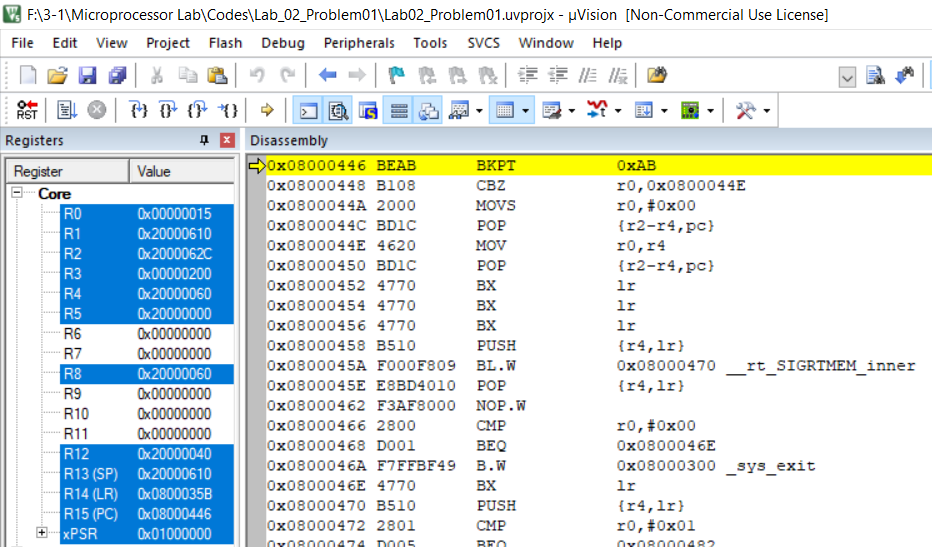
\includegraphics[width=1.1\textwidth]{problem01_01.png}
\end{center}

\subsubsection{After the Code has been Executed}
\begin{center}
    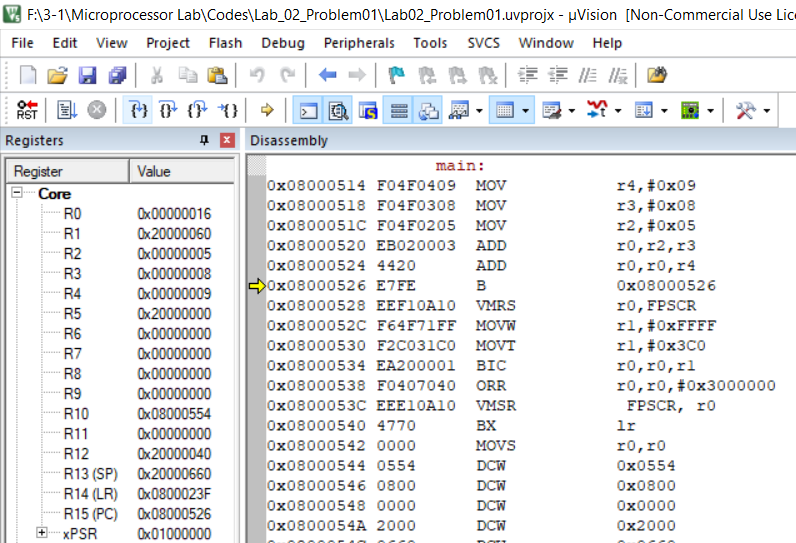
\includegraphics[width=1.1\textwidth]{problem01_02.png}
\end{center}

\section{Task 02}

\subsection{Detailed Code Explanation}

To solve this problem, I have first created three variables X, Y and Z with their initial values as X = 9, Y = 8 and Z = 5 by using the Opcode DCD. The DCD directive allocates one or more words of memory, aligned on four-byte boundaries, and defines the initial run-time contents of the memory. After this, in the main function I have used the Opcode LDR to load the register r4, r3 and r2 with the content of memory location of X, Y and Z respectively, thus r4 = X, r3 = Y and r2 = Z. We simply then add the values in the registers r2 and r3, and store the result in register r0 by using the Opcode ADD. Lastly, we again use the Opcode ADD to add the values in the registers r0 and r4, and store the final result in the register r0.

\subsection{Screenshot of Debugger}

\subsubsection{After the Code has been Loaded}
\begin{center}
    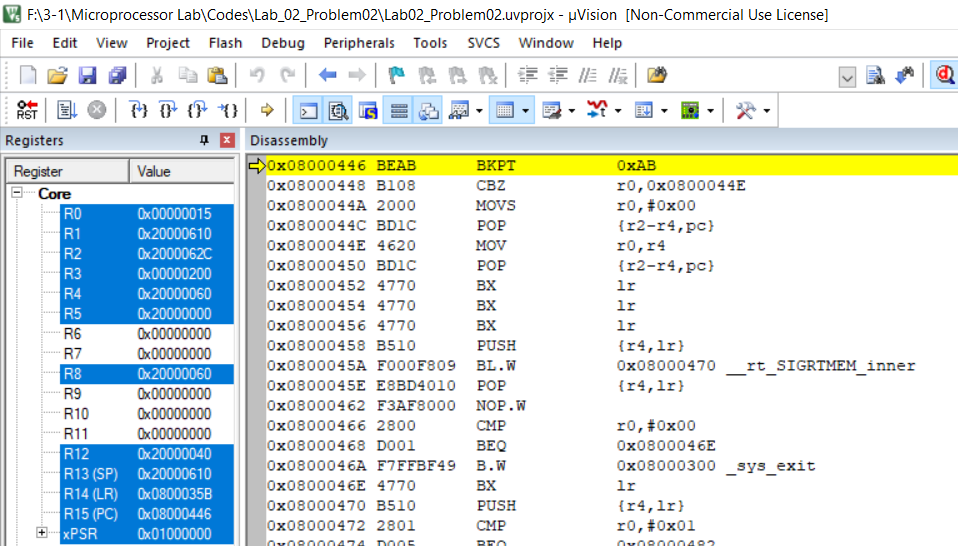
\includegraphics[width=1.1\textwidth]{problem02_01.png}
\end{center}

\subsubsection{After the Code has been Executed}
\begin{center}
    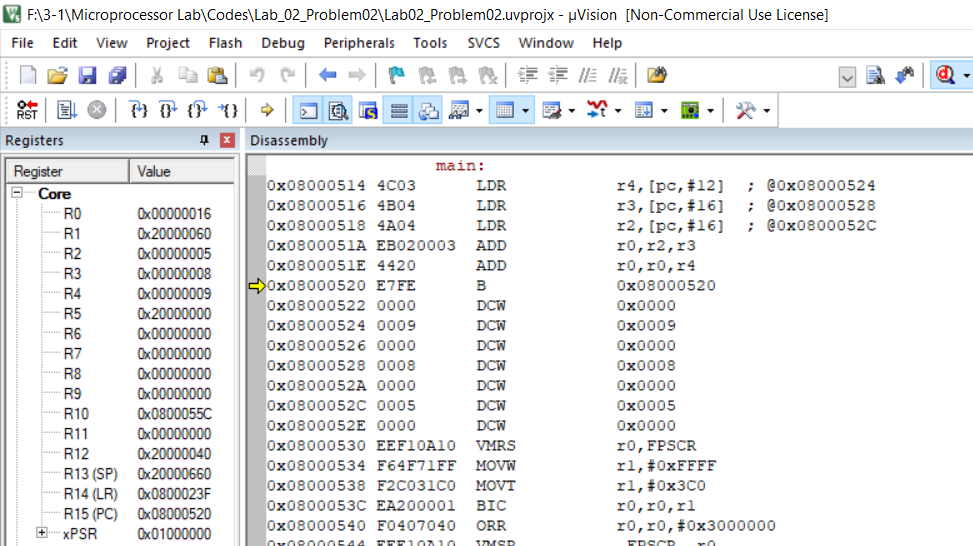
\includegraphics[width=1.1\textwidth]{problem02_02.png}
\end{center}

\section{Task 03}

\subsection{Detailed Code Explanation}

To solve this problem, I have first used the Opcode MOVW to load only 16 bits [15:0] to the registers r1 and r2 with the hexa-decimal values 0xFFFF. Then I have used the Opcode ADD to find the addition of the two 16 bit variables. Lastly, I have used the Opcode MOVT to load 0's in the upper 16 bit [31:16] of the final result, which is in register r0. Opcode MOVT writes to Rd[31:16], without affecting Rd[15:0]. Thus the required result is in the register r0.

\subsection{Screenshot of Debugger}

\subsubsection{After the Code has been Loaded}
\begin{center}
    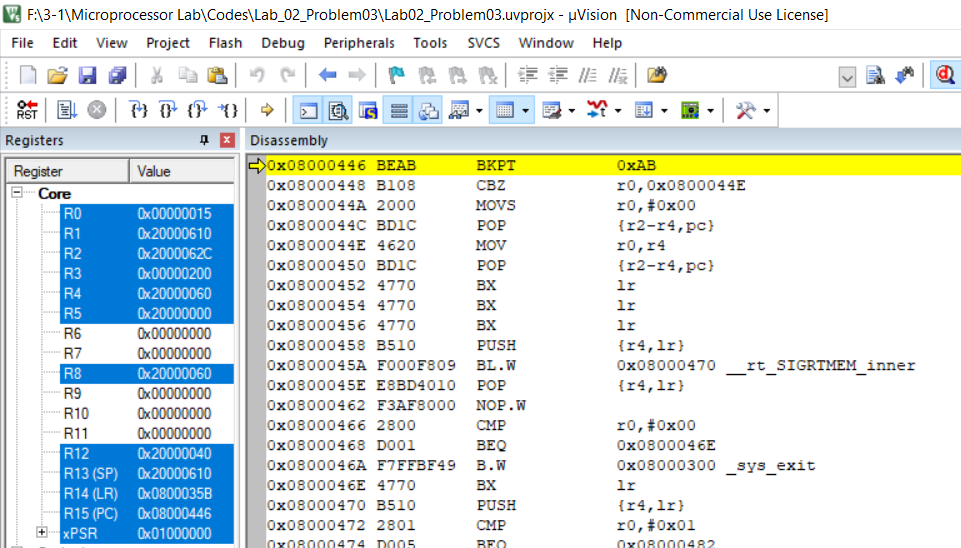
\includegraphics[width=1.1\textwidth]{problem03_01.png}
\end{center}

\subsubsection{After the Code has been Executed}
\begin{center}
    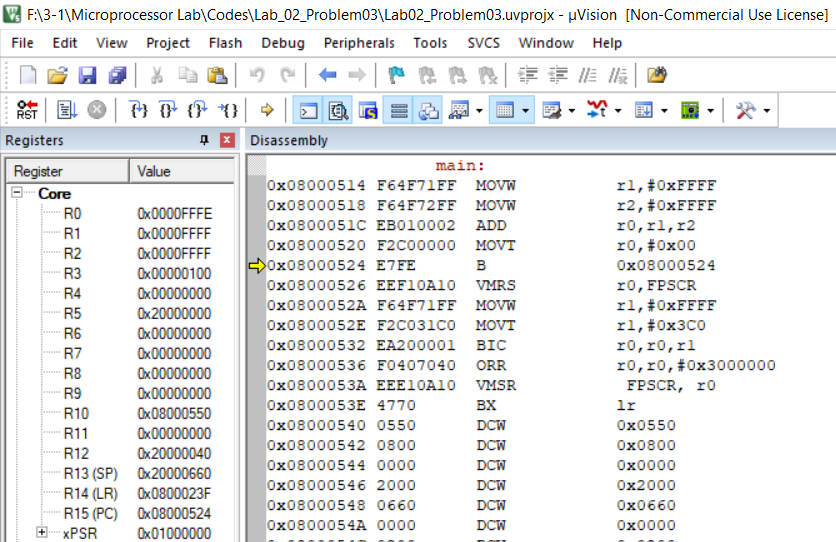
\includegraphics[width=1.1\textwidth]{problem03_02.png}
\end{center}

\section{Task 04}

\subsection{Detailed Code Explanation}

To solve this problem, I have first created two integer variables value1 and value2, and assigned their initial values as value1 = 8 and value2 = 9 by using the Opcode DCD. The DCD directive allocates one or more words of memory, aligned on four-byte boundaries, and defines the initial run-time contents of the memory. After this, in the main function I have used the Opcode LDR to load the register r1 and r2 with the content of memory location of value1 and value2 respectively, thus r1 = value1 and r2 = value2. To compare the values of these two registers I have used the Opcode CMP. The Opcode CMP compares the two operands. The BLT (branch less than) instruction is one of several conditional branch instructions. The conditional transfer instruction BLT transfers control to the statement labeled "done" if the contents of r1 contains the smaller integer number. Otherwise, the next instruction is executed. At "done", register r0 will always contain the smaller of the two integer numbers as the final result.

\subsection{Screenshot of Debugger}

\subsubsection{After the Code has been Loaded}
\begin{center}
    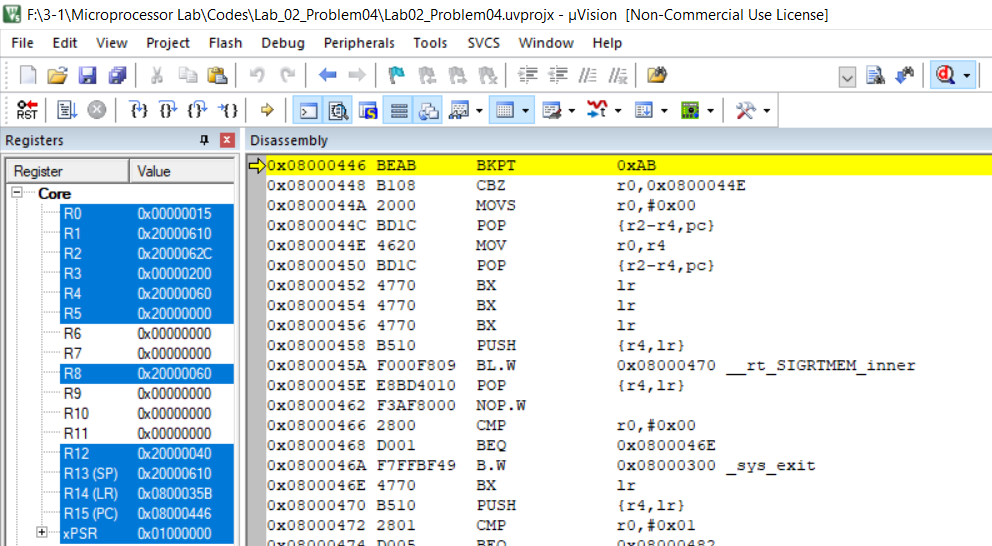
\includegraphics[width=1.1\textwidth]{problem04_01.png}
\end{center}

\subsubsection{After the Code has been Executed}
\begin{center}
    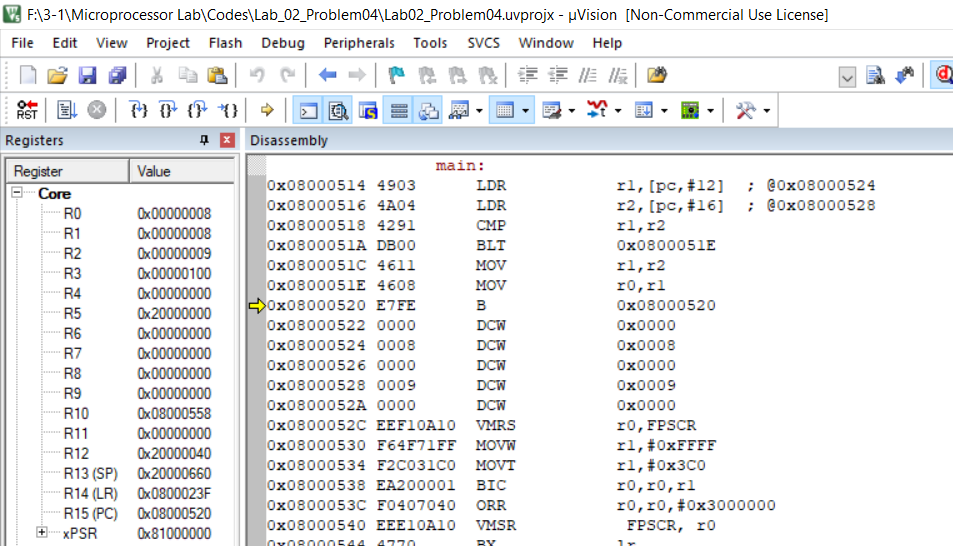
\includegraphics[width=1.1\textwidth]{problem04_02.png}
\end{center}

\end{document}